\documentclass[aspectratio=169]{beamer}

% ============================================
% HOOK BAZAAR THEME - MATCHING UI AESTHETICS
% ============================================
% Colors from client2/src/index.css:
% --color-primary: gold (#FFD700)
% --color-bg-darkest: #000814 (deep navy)
% --color-bg-dark: #001f3f (navy)
% --color-secondary: #003366
% --color-accent: #e85a4f (coral/terracotta)
% --color-white: #fff

\usepackage{fontspec}
\usepackage{tikz}
\usetikzlibrary{positioning}
\usepackage{graphicx}
\usepackage{booktabs}
\usepackage{hyperref}
\usepackage{fontawesome5}

% Define Hook Bazaar colors
\definecolor{hbPrimary}{HTML}{FFD700}      % Gold
\definecolor{hbBgDarkest}{HTML}{000814}    % Deep Navy
\definecolor{hbBgDark}{HTML}{001F3F}       % Navy
\definecolor{hbSecondary}{HTML}{003366}    % Secondary Blue
\definecolor{hbAccent}{HTML}{E85A4F}       % Coral/Terracotta
\definecolor{hbWhite}{HTML}{FFFFFF}        % White
\definecolor{hbMarble}{HTML}{F5F5F0}       % Marble Light

% Beamer theme configuration
\usetheme{default}
\usecolortheme{default}

% Set background and foreground
\setbeamercolor{background canvas}{bg=hbBgDarkest}
\setbeamercolor{normal text}{fg=hbWhite}
\setbeamercolor{frametitle}{fg=hbPrimary}
\setbeamercolor{title}{fg=hbPrimary}
\setbeamercolor{subtitle}{fg=hbWhite}
\setbeamercolor{author}{fg=hbMarble}
\setbeamercolor{date}{fg=hbMarble}
\setbeamercolor{item}{fg=hbPrimary}
\setbeamercolor{subitem}{fg=hbAccent}
\setbeamercolor{block title}{fg=hbBgDarkest, bg=hbPrimary}
\setbeamercolor{block body}{fg=hbWhite, bg=hbSecondary}
\setbeamercolor{structure}{fg=hbPrimary}

% Remove navigation symbols
\setbeamertemplate{navigation symbols}{}

% Custom frame title with gold underline
\setbeamertemplate{frametitle}{
    \vspace{0.5cm}
    {\Large\bfseries\insertframetitle}
    \vspace{0.1cm}
    \par
    \textcolor{hbPrimary}{\rule{\textwidth}{2pt}}
    \vspace{0.3cm}
}

% Custom footline
\setbeamertemplate{footline}{
    \hbox{%
    \begin{beamercolorbox}[wd=.333333\paperwidth,ht=2.25ex,dp=1ex,left]{author in head/foot}%
        \hspace*{2ex}\textcolor{hbPrimary}{\tiny Hook Bazaar}
    \end{beamercolorbox}%
    \begin{beamercolorbox}[wd=.333333\paperwidth,ht=2.25ex,dp=1ex,center]{title in head/foot}%
        \textcolor{hbMarble}{\tiny\insertshorttitle}
    \end{beamercolorbox}%
    \begin{beamercolorbox}[wd=.333333\paperwidth,ht=2.25ex,dp=1ex,right]{date in head/foot}%
        \textcolor{hbMarble}{\tiny\insertframenumber{} / \inserttotalframenumber}\hspace*{2ex}
    \end{beamercolorbox}}%
    \vskip0pt%
}

% Custom itemize
\setbeamertemplate{itemize item}{\textcolor{hbPrimary}{\faAngleRight}}
\setbeamertemplate{itemize subitem}{\textcolor{hbAccent}{\faAngleDoubleRight}}

% Fonts - Space Grotesk style (use system sans as fallback)
\setsansfont{Inter}[
    BoldFont={Inter Bold},
    Scale=1.0
]

% Title and content
\title{\textbf{Hook Bazaar}}
\subtitle{Decentralized Marketplace for Uniswap v4 Hooks}
\author{UHI7 Team}
\date{December 2025}

\begin{document}

% ============================================
% SLIDE 1: TITLE / INTRO
% ============================================
\begin{frame}
\begin{center}
\vspace{1cm}
{\Huge\textcolor{hbPrimary}{\textbf{Hook Bazaar}}}

\vspace{0.5cm}

\textcolor{hbMarble}{\large Decentralized Marketplace for Uniswap v4 Hooks}

\vspace{1.5cm}


\begin{tikzpicture}
    \draw[hbPrimary, line width=2pt] (-4,0) -- (4,0);
\end{tikzpicture}

\vspace{1cm}

\textcolor{hbWhite}{Building the Infrastructure Layer for the}\\[0.3cm]
\textcolor{hbPrimary}{\textbf{Uniswap v4 Hooks Economy}}

\vspace{1.5cm}

{\small\textcolor{hbMarble}{UHI7 Team $\cdot$ December 2025}}
\end{center}
\end{frame}

% ============================================
% SLIDE 2: PROBLEM / CHALLENGES
% ============================================
\begin{frame}{The Problem: 9 Critical Market Failures}

\begin{columns}[T]
\begin{column}{0.48\textwidth}
\textcolor{hbAccent}{\textbf{Market Infrastructure}}
\begin{itemize}
    \item \textbf{No marketplace} for hooks
    \item Supply \& demand exist --- no connection
    \item No competition mechanism
\end{itemize}

\vspace{0.5cm}

\textcolor{hbAccent}{\textbf{Developer Pain Points}}
\begin{itemize}
    \item No monetization model
    \item No IP protection (code is public)
    \item No reputation system
\end{itemize}
\end{column}

\begin{column}{0.48\textwidth}
\textcolor{hbAccent}{\textbf{Protocol Barriers}}
\begin{itemize}
    \item Custom hooks: \textcolor{hbPrimary}{\$10k--\$100k+}
    \item Development time: \textcolor{hbPrimary}{weeks--months}
    \item High audit costs \& risk
\end{itemize}

\vspace{0.5cm}

\textcolor{hbAccent}{\textbf{Ecosystem Gaps}}
\begin{itemize}
    \item No standardization
    \item No multi-hook composition
    \item Unsustainable economics
\end{itemize}
\end{column}
\end{columns}

\vspace{0.8cm}

\begin{center}

\begin{tikzpicture}
    \node[draw=hbAccent, thick, rounded corners, fill=hbSecondary, text=hbWhite, inner sep=10pt] {
        \textbf{Result:} Despite v4's power, the ecosystem lacks infrastructure for adoption
    };
\end{tikzpicture}
\end{center}
\end{frame}

% ============================================
% SLIDE 3: SOLUTION OVERVIEW
% ============================================
\begin{frame}{The Solution: Hook Bazaar}

\begin{center}
\textcolor{hbPrimary}{\large\textbf{A Decentralized Marketplace \& Infrastructure Layer}}
\end{center}

\vspace{0.5cm}

\begin{columns}[T]
\begin{column}{0.32\textwidth}
\begin{block}{\faCode\ For Developers}
\begin{itemize}
    \item Direct monetization
    \item IP protection via FHE
    \item Reputation profiles
    \item Professional exposure
\end{itemize}
\end{block}
\end{column}

\begin{column}{0.32\textwidth}
\begin{block}{\faBuilding\ For Protocols}
\begin{itemize}
    \item Instant deployment
    \item \textcolor{hbPrimary}{\$100s} vs \$10k+
    \item Pre-audited hooks
    \item Multi-hook composition
\end{itemize}
\end{block}
\end{column}

\begin{column}{0.32\textwidth}
\begin{block}{\faGlobe\ For Ecosystem}
\begin{itemize}
    \item Self-sustaining model
    \item Quality via competition
    \item Network effects
    \item V4 adoption boost
\end{itemize}
\end{block}
\end{column}
\end{columns}

\vspace{0.8cm}

\begin{center}
\textcolor{hbMarble}{Time-to-market: \textcolor{hbAccent}{\textbf{weeks}} $\rightarrow$ \textcolor{hbPrimary}{\textbf{minutes}}}
\end{center}
\end{frame}

% ============================================
% SLIDE 4: SOLUTION APPROACH
% ============================================
\begin{frame}{Architecture \& Approach}

\begin{center}
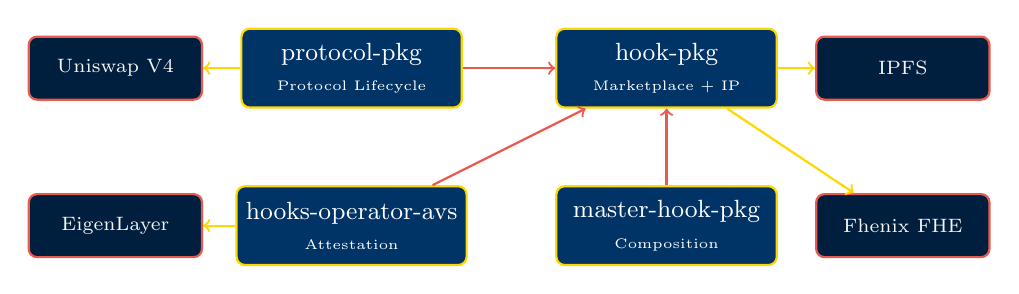
\begin{tikzpicture}[
    box/.style={draw=hbPrimary, thick, rounded corners=3pt, fill=hbSecondary, text=hbWhite, minimum width=2.8cm, minimum height=1cm, align=center, font=\small},
    external/.style={draw=hbAccent, thick, rounded corners=3pt, fill=hbBgDark, text=hbMarble, minimum width=2.2cm, minimum height=0.8cm, align=center, font=\scriptsize},
    arrow/.style={->, thick, hbPrimary}
]
    % Core packages
    \node[box] (protocol) at (0,2) {protocol-pkg\\{\tiny Protocol Lifecycle}};
    \node[box] (hook) at (4,2) {hook-pkg\\{\tiny Marketplace + IP}};
    \node[box] (avs) at (0,0) {hooks-operator-avs\\{\tiny Attestation}};
    \node[box] (master) at (4,0) {master-hook-pkg\\{\tiny Composition}};

    % External systems
    \node[external] (uniswap) at (-3,2) {Uniswap V4};
    \node[external] (eigen) at (-3,0) {EigenLayer};
    \node[external] (ipfs) at (7,2) {IPFS};
    \node[external] (fhenix) at (7,0) {Fhenix FHE};

    % Arrows
    \draw[arrow] (protocol) -- (uniswap);
    \draw[arrow] (avs) -- (eigen);
    \draw[arrow] (hook) -- (ipfs);
    \draw[arrow] (hook) -- (fhenix);
    \draw[arrow, hbAccent] (protocol) -- (hook);
    \draw[arrow, hbAccent] (avs) -- (hook);
    \draw[arrow, hbAccent] (master) -- (hook);
\end{tikzpicture}
\end{center}

\vspace{0.5cm}

\begin{columns}[T]
\begin{column}{0.48\textwidth}
\textcolor{hbPrimary}{\textbf{Core Packages}}
\begin{itemize}
    \item \textbf{protocol-pkg}: Pool administration
    \item \textbf{hook-pkg}: Development \& marketplace
    \item \textbf{hooks-operator-avs}: EigenLayer attestation
    \item \textbf{master-hook-pkg}: Diamond composition
\end{itemize}
\end{column}

\begin{column}{0.48\textwidth}
\textcolor{hbPrimary}{\textbf{Sponsor Integrations}}
\begin{itemize}
    \item \textbf{Fhenix CoFHE}: Encrypted hooks for IP protection
    \item \textbf{EigenLayer AVS}: Cryptoeconomic guarantees via staked operators
\end{itemize}
\end{column}
\end{columns}
\end{frame}

% ============================================
% SLIDE 5: FEATURE 1 - HOOK SPECIFICATION FORMAT
% ============================================
\begin{frame}{Key Feature: Mathematical Hook Specifications}

\begin{columns}[T]
\begin{column}{0.55\textwidth}
\textcolor{hbPrimary}{\large\textbf{Hook Specification Format (HSF)}}

\vspace{0.3cm}

\textcolor{hbAccent}{\textbf{Why It Matters}}
\begin{itemize}
    \item Objective behavior verification
    \item Formal state machine definitions
    \item Machine-readable specifications
    \item Foundation for AVS attestation
\end{itemize}

\vspace{0.5cm}

\textcolor{hbAccent}{\textbf{What It Enables}}
\begin{itemize}
    \item \textbf{Trust}: Verify before integrating
    \item \textbf{Comparison}: Objective evaluation
    \item \textbf{Slashing}: Proof of misbehavior
    \item \textbf{Composition}: Safe multi-hook stacking
\end{itemize}
\end{column}

\begin{column}{0.42\textwidth}
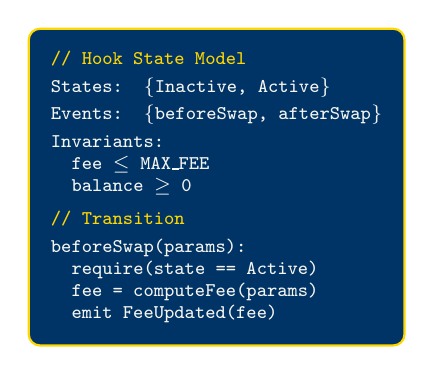
\begin{tikzpicture}
    \node[draw=hbPrimary, thick, fill=hbSecondary, text=hbMarble, rounded corners, inner sep=8pt, font=\scriptsize, align=left] {
        \textcolor{hbPrimary}{\texttt{// Hook State Model}}\\[2pt]
        \texttt{States: \{Inactive, Active\}}\\[2pt]
        \texttt{Events: \{beforeSwap, afterSwap\}}\\[2pt]
        \texttt{Invariants:}\\
        \texttt{\ \ fee $\leq$ MAX\_FEE}\\
        \texttt{\ \ balance $\geq$ 0}\\[4pt]
        \textcolor{hbPrimary}{\texttt{// Transition}}\\[2pt]
        \texttt{beforeSwap(params):}\\
        \texttt{\ \ require(state == Active)}\\
        \texttt{\ \ fee = computeFee(params)}\\
        \texttt{\ \ emit FeeUpdated(fee)}
    };
\end{tikzpicture}

\vspace{0.3cm}

\begin{center}
\textcolor{hbMarble}{\scriptsize Specifications stored on IPFS}\\
\textcolor{hbMarble}{\scriptsize Verified by EigenLayer operators}
\end{center}
\end{column}
\end{columns}
\end{frame}

% ============================================
% SLIDE 6: FEATURE 2 - AVS ATTESTATION
% ============================================
\begin{frame}{Key Feature: EigenLayer AVS Attestation}

\begin{columns}[T]
\begin{column}{0.55\textwidth}
\textcolor{hbPrimary}{\large\textbf{Cryptoeconomic Guarantees}}

\vspace{0.3cm}

\textcolor{hbAccent}{\textbf{Why It Matters}}
\begin{itemize}
    \item Staked operators verify hook behavior
    \item Economic penalties for false attestations
    \item Decentralized trust --- no central authority
    \item Continuous compliance monitoring
\end{itemize}

\vspace{0.5cm}

\textcolor{hbAccent}{\textbf{Slashing Mechanism}}
\begin{itemize}
    \item \textbf{50\% slash}: False positive attestation
    \item \textbf{30\% slash}: False negative (missed violation)
    \item Challenge window for disputes
    \item Proof submitted on-chain
\end{itemize}
\end{column}

\begin{column}{0.42\textwidth}
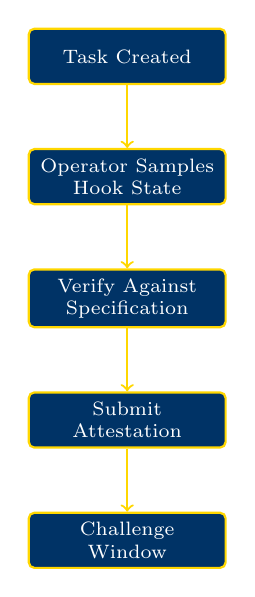
\begin{tikzpicture}[
    node distance=0.8cm,
    box/.style={draw=hbPrimary, thick, rounded corners=2pt, fill=hbSecondary, text=hbWhite, minimum width=2.5cm, minimum height=0.7cm, align=center, font=\scriptsize},
    arrow/.style={->, thick, hbPrimary}
]
    \node[box] (task) {Task Created};
    \node[box, below=of task] (sample) {Operator Samples\\Hook State};
    \node[box, below=of sample] (verify) {Verify Against\\Specification};
    \node[box, below=of verify] (attest) {Submit\\Attestation};
    \node[box, below=of attest] (challenge) {Challenge\\Window};

    \draw[arrow] (task) -- (sample);
    \draw[arrow] (sample) -- (verify);
    \draw[arrow] (verify) -- (attest);
    \draw[arrow] (attest) -- (challenge);
\end{tikzpicture}

\vspace{0.3cm}

\begin{center}
\textcolor{hbMarble}{\scriptsize Powered by EigenLayer restaking}
\end{center}
\end{column}
\end{columns}
\end{frame}

\end{document}
